\chapter{Projektowanie i implementacja}
\label{cha:implementacja}

Nakreślony problem -- rozproszonego systemu, który dzięki propagacji danych między użytkownikami obniży obciążenie serwerów sieci Web -- stawia wiele wyzwań projektowych i architektonicznych.

\section{Wymagania funkcjonalne}
\label{sec:funkcjonalnosc}

System dHTTP, z punktu widzenia użytkownika, ma spełniać jedną funkcjonalność: utrzymać lub poprawić płynność dostępu do interesujących go witryn internetowych, nie wpływając na ich treść i nie naruszając prywatności.

Projekt udostępnia interfejs zapewniający dostęp do statystyk, a także preferencji użytkownika. Udostępnione preferencje dotyczą: stopnia działania aplikacji w tle, trybów propagacji i przechowywania danych.
% To może powinno być gdzieś indziej
\begin{figure}[h]
	\centering
    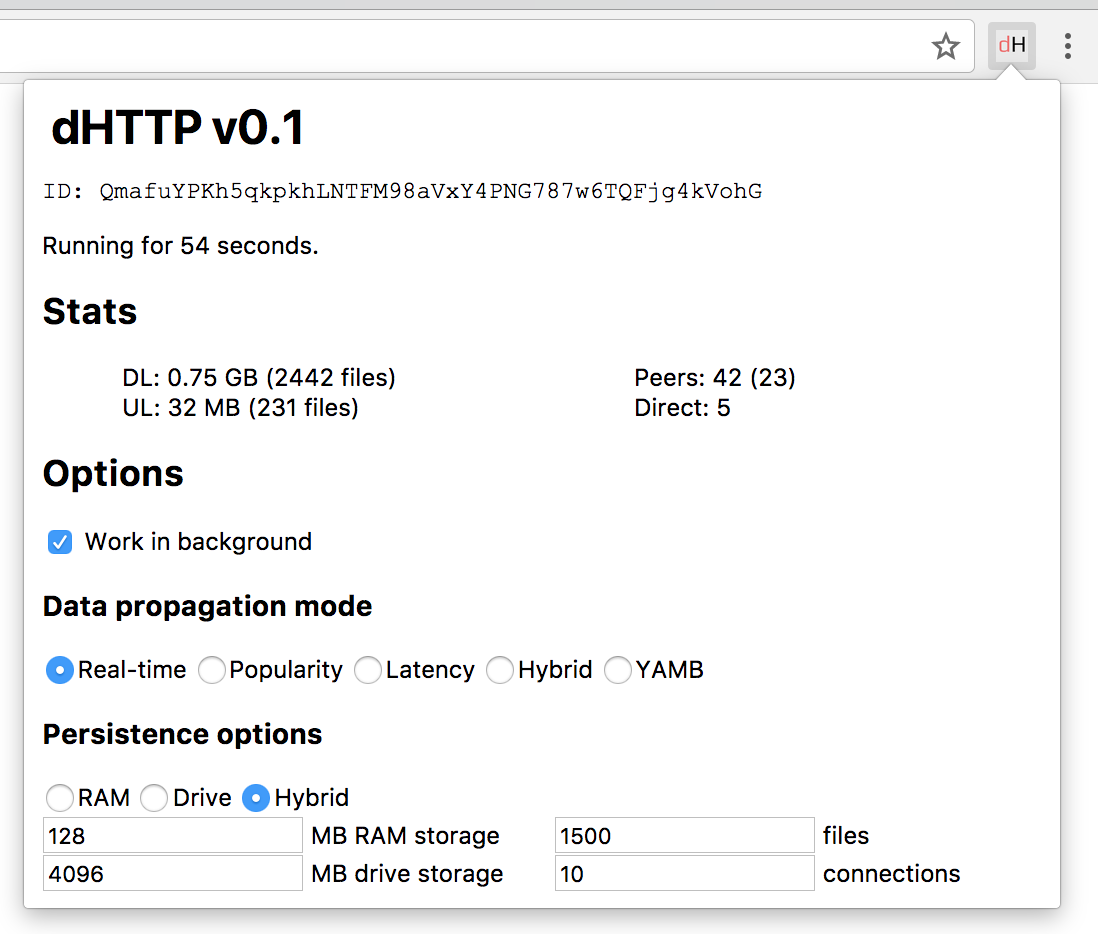
\includegraphics[scale=0.5]{dhttp-initial-interface.png}
	
	\caption{\label{fig:initialInterface} Wstępna implementacja interfejsu operacji dla systemu dHTTP: pop-up dostarczany przez wtyczkę do przeglądarki Google Chrome pozwala na obserwację statystyk i zmianę preferencji.}
\end{figure}

% TODO - gdzieś w pracy podkreśl, jak bardzo istotna jest prosta i automatyczna klastryzacja
Wymogiem dla projektu, koniecznym z racji potrzeby prostej automatyzacji rozrostu sieci, jest tryb niezależny aplikacji -- {\em headless mode} -- pozwalający na wystartowanie niezależnego węzła jednym poleceniem. Istotnym jest, aby węzeł tego typu udostępniał statystyki użycia i wstępną konfigurację przy użyciu poleceń interfejsu konsolowego, pozwalając jednak na funkcjonalne uruchomienie z domyślną konfiguracją.


\section{Definicje, architektura i technologie}
\label{sec:zalozeniaProjektu}

\subsection{Słownik pojęć}

W celu uniknięcia niejednoznaczności w dalszym toku pracy, zdefiniowane zostaną następujące pojęcia:

\begin{itemize}
    \item \textbf{węzeł} -- pojedynczy, autonomiczny element systemu, który wykorzystuje komunikację sieciową w celu rozgłaszania i pobierania danych;
    \item \textbf{klient} -- węzeł, który pobiera dane w celach użytkowych, zaimplementowany w wersji dedykowanej użytkownikowi końcowemu;
    \item \textbf{klaster} -- zbiór węzłów, który posiada informacje i ścieżki komunikacyjne pozwalające efektywnie na wymianę informacji pomiędzy każdym z nich;
    \item \textbf{metadane klastra} -- ustrukturyzowane informacje wymieniane pomiędzy węzłami w celu ustalenia stanu i optymalizacji działania klastra;
    \item \textbf{metadane pliku} -- ustrukturyzowane informacje wymieniane między węzłami w celu propagacji i umożliwienia wymiany faktycznych danych plikowych;
\end{itemize}
      % TODO - dodać nowe, jeśli się pojawią/przyjdą do głowy

\subsection{Koncept architektury}

Z punktu widzenia klastra, koncepty węzła i klienta są jednoznaczne i równorzędne -- wszystkie wyposażone są we wspólne mechanizmy komunikacji, i protokół wymiany danych między nimi działa na niezmienionej zasadzie. Wspólnie budować będą rozproszoną tablicę haszującą (DHT), która pozwoli na dostęp do metadanych klastra informujących o cechach poszczególnych węzłów oraz metadanych plików, przyspieszając proces ich identyfikacji i zapewniając bezpieczeństwo oraz spójność danych.

W celu zapewnienia płynności działania systemu, metadane klastra powinny zawierać w sobie informacje o {\em reputacji} poszczególnych węzłów. Podczas gdy węzły serwerowe z reguły zostają uruchomione i będą działać, mając szczyty obciążenia czy wymagań zależne głównie od obciążenia całej sieci (lub ewentualnego alternatywnego oprogramowania serwerowego na nich uruchamianego), węzły klienckie podlegać będą prawdopodobnie o wiele większej dynamice, z racji licznych odczytów dużych plików i podejścia użytkownika, które może zakładać częste otwieranie i zamykanie przeglądarki.

Węzły serwerowe i klienci powinny mieć zatem różne wartości bazowe przy ocenie ich sprawności w sieci -- reputacja oprogramowania klienckiego powinna być domyślnie niższa, i szybciej reagować na zmiany jej wartości.

\subsection{Wykorzystane technologie i narzędzia}
\label{sec:techNTools}
% akapit poniżej prawdopodobnie jest o wiele lepszą kanwą dla czegoś w części teoretycznej niż czymś, co powinno być tutaj.

Budowa kompletnego stosu technologicznego dla projektu o takich wymaganiach przez lata pozostawała problemem nietrywialnym. Paradygmaty programowania specjalizowane w podejściu obiektowym wspierały budowę monolitów, a komunikacja klient-serwer często polegała na tworzeniu dużej ilości poleceń, bez skupienia na wydajności takich rozwiązań.

Dużą zmianą w tej kwestii jest rozwój \texttt{libp2p}, stanowiący efekt długotrwałej pracy nad zrozumieniem stosu sieciowego Internetu, zbiór protokołów i wyprowadzonych zeń narzędzi, mechanik i interfejsów, pozwalających na ich podstawie budować własne, kompleksowe rozwiązania (\cite{libp2p-specs}).

\texttt{libp2p} stanowi względnie wysokopoziomową kanwę dla projektu dHTTP. To właśnie na efektach pracy tego projektu opiera się warstwa tworzenia i komunikacji węzłów, budująca klaster dHTTP. Implementacja \texttt{js-libp2p} udostępnia moduły niezbędne w komunikacji sieciowej, łączeniu strumieni różnych protokołów, wykrywaniu nowych węzłów, propagowaniu informacji o stanie sieci czy wreszcie budowaniu rozproszonej tablicy haszującej, stanowiącej bazę metadanych klastra i plików.

Nie bez wpływu pozostaje rozwój przeglądarek internetowych. Współczesne browsery udostępniają kompleksowe API, pozwalające rozwijać wtyczki zmieniające zawartość stron internetowych, z uwzględnieniem kwestii wydajności i bezpieczeństwa. Istotne jest również wsparcie dla nowych technik komunikacji takich jak {\em WebSockets}, pozwalającej na wymianę informacji w czasie rzeczywistym, dzięki utrzymywaniu dwustronnie interaktywnej sesji TCP pomiędzy przeglądarką i serwerem. W ramach tej pracy rozwinięta została wtyczka dla przeglądarki Google Chrome. Wybór ten podyktowany został znaczną przewagą Chrome -- w chwili pisania tej pracy, udział Chrome w rynku przeglądarek na komputerach osobistych wynosił ponad 64\% (\cite{chromeStats}). Prace i testy przeprowadzono przy użyciu 64-bitowego Google Chrome w wersji 63.0, na platformie macOS w wersji 10.13.2.
% TODO cite https://developer.chrome.com/extensions lub bardziej specyficznie.

Za powstanie {\em headless} dHTTP w znacznej części odpowiada Node.js -- środowisko uruchomieniowe pozwalające na uruchamianie kodu JavaScript po stronie serwerowej.  Narzędzia, takie jak \texttt{npm} i Browserify, pozwalają z kolei na wykorzystywanie serwerowego kodu JavaScriptu w kodzie klienckim. Dzięki możliwości rozwoju obu aplikacji przy użyciu tego samego języka programowania i powyższym rozwiązaniom, znaczna część  kodu aplikacji może być współdzielona. {\em Headless} dHTTP testowane było przy użyciu \texttt{node} w wersji v8.9.1, na platformie macOS oraz Amazon Linux AMI.

% Języki programowania nie były zaadaptowane do prostej komunikacji sieciowej, a przeglądarki nie wspierały krytycznych narzędzi i protokołów pozwalających na komunikację w czasie rzeczywistym, pozostawiając problemy natury wydajnościowej uniemożliwiające użyteczną implementację tego typu rozwiązań.

\subsection{Paradygmaty i koncepcje}
Istotą projektu dHTTP jest reagowanie na zapytania i komunikacja pomiędzy węzłami. Ponadto, projekt działać będzie w środowisku JavaScriptowym -- język ten (poza web workers -- rozwiązaniem polegającymi na delegacji obliczeń do wydzielonego środowiska, patrz: \cite{webWorkers}) uruchamiany jest jednowątkowo. W podejściu proceduralnym może to powodować problemy związane z blokowaniem się wydarzeń; jest to dotkliwe zwłaszcza w przypadku interfejsów użytkownika, które w takiej sytuacji tracą responsywność. Poniższe sekcje zawierają omówienie związanym z tych praktyk, stosowanych w projekcie dHTTP.
% TODO - podkreśl jak pozytywny wpływ ma to wszystko na sposób pisania dHTTP

\subsubsection{Asynchroniczność}
Podstawowym rozwiązaniem stosowanym w języku JavaScript, pozwalającym na wykonanie w środowisku jednowątkowym, jest model współbieżności oparty o tzw {\em event loop}. Wywołania funkcji odkładane są na stosie, podczas gdy kolejne wiadomości są wkładane do kolejki FIFO. Podstawowym założeniem jest nigdy nie blokować -- jeśli jakieś wywołanie wymaga konkretnej reakcji, definiowanej przez użytkownika, należy nasłuchiwać wydarzeń lub użyć wywołań zwrotnych (\texttt{callback}).

\begin{lstlisting}[language=javascript]
    function foo(callback) {
        var a = someWaitingOperation()
        callback(a)
    }

    foo((a) => print(a))
    console.log('Hello, world!')
\end{lstlisting}

W powyższym przykładzie warto zauważyć, że wywołanie \texttt{console.log(...)} będzie miało miejsce natychmiast po zawołaniu funkcji foo -- jest więc bardzo prawdopodobnym, że efekt jego pracy widoczny będzie przed zawołaniem funkcji \texttt{callback}.

Asynchroniczne odwołania są kluczowe w przypadku wydarzeń takich jak oczekiwanie na odpowiedź serwera; czekając, program może wykonywać następne polecenia, a reakcja na odpowiedź zostanie wpleciona w tok pracy aplikacji.

\subsubsection{Event-driven architecture}
Pozioma oś modelu współbieżności JavaScriptu zapewnia natywne wsparcie dla reakcji na wydarzenia. W celu nasłuchiwania wydarzenia, należy zarejestrować jego obserwatora ({\em listener}) stosując z reguły składnię zbliżoną do:
\begin{lstlisting}[language=javascript]
    a.addEventListener('click', ()=> {
        console.log('Button clicked!')
    })
\end{lstlisting}

W powyższym przykładzie, widać rejestrację reakcji na kliknięcie w przycisk. Jeżeli dana sytuacja nastąpi, wiadomość wysłana zostanie na kolejkę, co w momencie jej napotkania doprowadzi do wrzucenia na stos zarejestrowanej funkcji.

\begin{figure}[h]

    \centering
    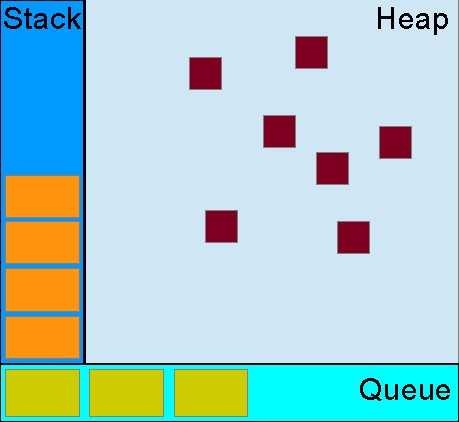
\includegraphics[scale=0.6]{js-concurrency.pdf}
    % \subcaption{\label{subfigure_a}}

	\caption{Wizualizacja modelu współbieżności języka JavaScript -- widać stos funkcji (oś pionowa) i kolejkę wydarzeń (oś pozioma). Pomiędzy nimi znajduje się współdzielona sterta, zapewniająca dostęp do danych. Źródło: \cite{eventLoop}}

\end{figure}

\subsubsection{Strumienie}
% i potoki

Node.js przeniósł środowisko JavaScript, którego dotychczasowym targetem były lekkie rozwiązania klienckie, na poziom serwerowy, w którym niektóre operacje są długotrwałe, mają przerwy w wywołaniach i nierzadko wymagają informowania o postępach (przykładem może być utrzymanie połączenia sieciowego, czy odczyt standardowego wyjścia). Choć jest możliwym implementacja tego typu rozwiązań  wywołaniami zwrotnymi, czytelność i utrzymywalność takiego kodu drastycznie spada -- przepływ logiki programu staje się trudny do wyśledzenia.

Z pomocą przychodzą strumienie (\cite{nodeStreamAPI}). Strumienie nakładają abstrakcję, która pozwala intuicyjnie czytać (dla strumieni \texttt{Readable}) wrzucać (w przypadku \texttt{Writable}), a także transformować (\texttt{Transform}) przekazywane wartości.

\begin{lstlisting}[language=javascript]
// Przykład nawiązywania połączenia w metaprotokole dHTTP
dhttpClient.node.dial(peerInfo, '/dhttp/meta/0.1', (err, connStream) => {
    // connStream to przykład strumienia Duplex - pozwala zarówno na zapis, jak i odczyt.
    // zapis do connStream
    connStream.write("Let's talk")
    // jeśli w strumieniu pojawią się dane, nastąpi wywołanie funkcji callback. Warto zauważyć, że to wywołanie może nastąpić zarówno przed, jak i po zawołaniu write -- zależy od stanu strumienia, który może otrzymywać dane w innych miejscach programu
    connStream.on('data', (data) => {
        callback(JSON.parse(data))
    })
}


// Przykład uruchamiania serwera HTTP w node.js dzięki 'http-server'
http.createServer((req, res) => {
    // Przekazanie strumienia req strumieniowi request, który następnie zostanie przekazany do res. W efekcie zadziałamy jako najprostsze proxy - otrzymamy dane o oryginalnym zapytaniu, wywołamy je z punktu widzenia serwera, i przekażemy wynik w ramach odpowiedzi.
    req.pipe(request(req.url)).pipe(res)
}).listen(34887)
\end{lstlisting}

Powyższy przykład, stanowiący część kodu dHTTP, pokazuje istotny koncept {\em potoków} (ang. {\em pipe}). Potoki pozwalają łączyć strumienie w sposób analogiczny do strumieni znanych z systemów Uniksowych: odczytane wartości można przekazać kolejnemu strumieniowi, który może zamienić je na inne wartości, aż w końcu wynik pracy zostanie zapisany w strumieniu odpowiedzi. Tego typu operacje stanowią kanwę przemian stosowanych w dHTTP.

Podkreślić należy również pozytywny wpływ strumieni na wydajność -- ta abstrakcja pozwala operować na plikach przy użyciu buforów w sposób przezroczysty: przykładowo, aby wysłać duży obrazek nie przechowując go w całości w pamięci, wystarczy utworzyć strumień pliku i przepotokować go do strumienia wyjściowego.

\begin{lstlisting}[language=javascript]
    var fileStream =  fs.createReadStream('files/caviar.jpg');
    fileStream.pipe(connStream)
    //kiedy strumień pliku się zakończy, nastąpi zamknięcie połączenia aby poinformować odbiorcę, że nic już na niego nie czeka
    fileStream.on('finish', ()=> connStream.close())
\end{lstlisting}


% W celu walki z zaimplementowano wiele rozwiązań, od 

% Jak Bóg da, to się napisze te rzeczy
% \subsubsection{Decentralizacja czy rozproszenie?}
% \label{sec:decentralizacjaCzyRozproszenie}

% \subsection{Bezpieczeństwo}
% \label{sec:security}

% \subsubsection{Czy autentykacja to nasza brożka?}
% \subsubsection{Gdzie leżą granice zdrowych heurystyk?}

% \subsection{Enkapsulacja}

% \subsection{Komunikacja}

% Z tego poniżej może powstać osobny rozdział, gdzie to co powyżej stanowiłoby bardziej rozważania na temat właściwego podejścia do realizacji projektu, a to poniżej -- faktyczny opis implementacji systemu, podzielony bardziej granularnie dla każdego z elemenetów

\section{Interfejs \texttt{dhttp.js}}

Podstawę logiki systemu stanowi plik \texttt{dhttp.js}. Jest on interfejsem łączącym backend i stronę użytkową, pozwalającym na dostęp do informacji na temat sposobu działania węzła, a także wykonywanie operacji w sieci dHTTP.

\texttt{dhttp.js} operuje na dwóch protokołach:

\begin{itemize}
    \item \texttt{/dhttp/meta/0.1} -- {\em metaprotokół}, stanowi podstawę szkieletu systemu dHTTP. Informuje o dostępnych węzłach i plikach, obciążeniu sieci, a także następujących na bieżąco zmianach. Konwencją podjętą dla {\em metaprotokołu} jest powszechna propagacja danych -- przykładowo, jeśli następuje połączenie z nowym węzłem,  należy wysłać mu listę posiadanych plików, a jeśli planowane jest opuszczenie sieci, trzeba poinformować o tym fakcie podłączonych sąsiadów. Dzięki temu podejściu każdy węzeł posiada zbiór informacji na temat otoczenia, pozwalający na szybsze podejmowanie decyzji.

    \item \texttt{/dhttp/data/0.1} -- {\em protokół danych}, stanowi system przesyłu docelowych plików w dHTTP. Zorientowany strumieniowo, przesyła zgromadzone pliki w ich oryginalnym formacie. Może zostać rozszerzony o obsługę zapytań cząstkowych -- tak, aby duże pliki pobierać częściami od swoich sąsiadów.
\end{itemize}
Ponadto, \texttt{dhttp.js} wykorzystuje wbudowane {\em mechanizmy odkryć} \texttt{libp2p} w celu wykrywania sąsiadów i zmian sieci.


% tutaj bardzo duże wypisanie wszystkich szczegółów jakie dają protokoły, z rysunkami i wszyściutkim

\subsection{Warstwa sieciowa}
Warto zaznaczyć, że rozwiązania opisywane w powyższej sekcji jako {\em protokół} są wysokopoziomową nakładką na warstwę sieciową. Jak zatem węzły nawiązują połączenie?
% rozwinąć wątek NAT-u

Połączenia w sieci peer-to-peer są znacznie utrudnione przez \textbf{ Network Address Translation} (NAT). NAT jest techniką stosowaną przez routery, polegającą na zmianie adresów i portów IP w toku przesyłu danych w celu udostępnienia węzłom sieci prywatnych dostępu do internetu przy użyciu jednego adresu. Gdy użytkownik za „maskaradą” (jak bywa określany NAT) wykonuje zapytania, serwery widzą adres IP pierwszego routera, który posiada publiczny adres sieciowy. Odpowiedzi są możliwe dzięki informacjom przechowywanym przez routery prowadzące ten typ komunikacji.

Jest to konieczność w obliczu wyczerpanej puli adresów IPv4, prowadzi jednak do sytuacji, w której otwarcie bezpośredniego łącza pomiędzy dwoma użytkownikami końcowymi jest z reguły niemożliwe -- nie ma możliwości odpytania adresu IP końcowego komputera.

W celu poradzenia sobie z tym problemem, dHTTP wykorzystuje bibliotekę \texttt{js-libp2p-webrtc-star}. To rozwiązanie działa na zasadzie serwera spotkań ({\em Rendezvous Server}), który stanowi swoisty przekaźnik i pozwala na rejestrację węzłów. Dzięki temu, jest jednocześnie odpowiedzialny za warstwę transportu jak i {\em mechanizm odkryć}.

\begin{figure}[h]
        \centering
        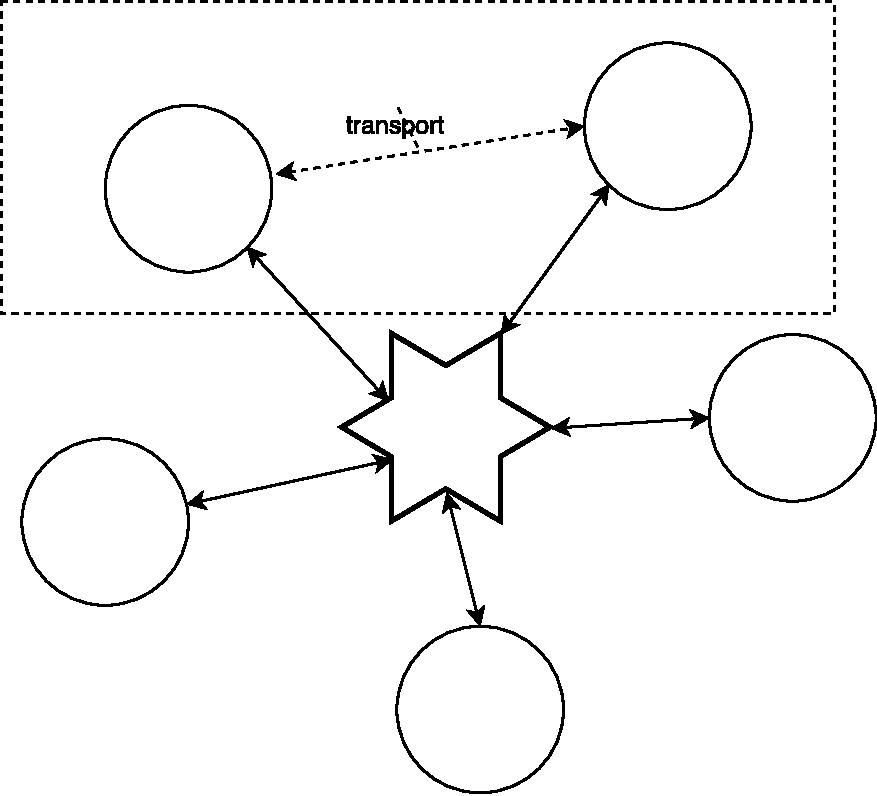
\includegraphics[scale=0.5]{webrtc-star.pdf}
        % \subcaption{\label{subfigure_a}}
    
        \caption{Wizualizacja sieci opartej o \texttt{js-libp2p-webrtc-star}, z przykładem wirtualnego połączenia transportowego pomiędzy dwoma węzłami.}
        \label{fig:webrtc-star}
\end{figure}

Niestety, stawia to pod znakiem zapytania rozproszenie systemu -- jak widać na rys. \ref{fig:webrtc-star}, obecnie system przypomina bardziej scentralizowaną topologię gwiazdy niż system faktycznie rozproszony. Obciąża też {\em Rendezvous Server} koniecznością przekazywania treści. Jest to jednak rozwiązanie przejściowe i na chwilę obecną konieczne -- \texttt{js-libp2p} w czasie tworzenia tego projektu nie udostępnia innych metod trawersowania NAT-u.

Warto dodać, że w przypadku sieci opartej wyłącznie o węzły w sieci lokalnej możliwe jest stosowanie tzw. Multicast DNS, który nie potrzebuje żadnego punktu centralnego; w przypadku serwerów posiadających publiczne adresy IP, możliwe staje się użycie list adresów utrzymywanych przez serwery śledzące -- trackery -- oba rozwiązania pozwalają na bezpośredni transport pomiędzy węzłami i nie wymagają zmiany logiki systemu (\cite{discoverylibp2p}).

\subsection{Struktura metadanych}

Metadane przesyłane przy użyciu \texttt{/dhttp/meta/0.1} to podstawa przepływu danych w systemie. Wykorzystywane do budowania wspólnej bazy wiedzy na temat sieci, składać się muszą z lekkich struktur i jasnych komunikatów.

Podstawowe zapytanie \texttt{/dhttp/meta/0.1} wygląda następująco:

\begin{lstlisting}[language=javascript]
    {
        type: "echo",
        peerId: dhttpClient.node.peerInfo.id.toB58String(),
        text: "Hello, node."
    }
\end{lstlisting}

Omówienie zapytań i odpowiedzi jest zawarte w rozdziale \ref{sec:api}.

\section{API}
\label{sec:api}

W tej sekcji szczegółowo opisane zostały udostępnione przez \texttt{dhttp.js} funkcje i mechanizmy związane ze strukturami i przepływami danych pomiędzy węzłami. Ogólny przepływ informacji systemu zawiera się w podsekcji \ref{sec:transportAlgorithm}, opisującej cykl życia węzła.

Podstawowym założeniem jest istnienie singletona\footnote{Możliwość tworzenia obiektu ograniczona jest do pojedynczej, globalnie dostępnej instancji.} \texttt{dhttpClient}, który przy rozruchu aplikacji inicjalizuje węzeł sieci. Wszelkie odwołania do działania węzła powinny polegać na rejestrowaniu wydarzeń i wywoływaniu funkcji globalnego obiektu \texttt{dhttpClient}.

\subsection{Struktury danych}
W celu poprawy wydajności i uproszczenia przepływów w aplikacji, dHTTP oferuje kilka struktur informujących o dostępności danych.

Typy struktur jak i funkcje oferowane przez \texttt{js-libp2p}, do których odnosi się poniższe API, opisane są na stronie projektu: \cite{libp2pReadme}.

\subsubsection{Struktury podstawowe}
\begin{itemize}
    \item \textbf{\texttt{PeerId}} -- \texttt{String} zawierający ID węzła sieci, uzyskane dzięki zawołaniu \texttt{PeerInfo.id.toB58String()}
    \item \textbf{\texttt{RequestURL}} -- \texttt{String} zawierający ścieżkę zapytania klienckiego. Jeśli klient odpyta nasz serwer na adresie \texttt{http://localhost:34887/http://example.com/script.js}, instancja \texttt{RequestURL} zawierać będzie \texttt{http://example.com/script.js}.
    \item \textbf{\texttt{popularityIndex}} -- \texttt{Integer} określający popularność danego pliku z perspektywy posiadającego go węzła.
    \item \textbf{\texttt{Data}} -- serializowalny obiekt zawierający dane przesyłane w ramach metaprotokołu, zgodne z formatami zdefiniowanymi w \ref{sub:metaprotocolMessages}.
\end{itemize}

% 

\subsubsection{\texttt{filesInNetwork}}
\begin{lstlisting}[language=javascript]
filesInNetwork: {
        "http://example.com/file.jpg": { // RequestURL
            nodes: {
                PeerId: {
                    popularityIndex: Int,
                }
            }
            popularityIndex: Int
        },
        "http://example.com/script.js" : {...}
    }
\end{lstlisting}
\texttt{filesInNetwork} jest strukturą odpytywaną przy połączeniu klienckim. Stanowi pierwszy punkt wejścia do sieci, i zoptymalizowany jest pod szybkie przeszukanie i weryfikację, czy plik jest dostępny przy użyciu dHTTP.

Poszczególne elementy indeksowane są poprzez adresy URL zasobów pobieranych przez klienta (\texttt{ReqestURL}).

\textbf{Pola:}
\begin{itemize}
    \item \textbf{\texttt{nodes}} -- mapa zawierająca informacje tych klientów, którzy posiadają dostęp do danego pliku.
    \item \textbf{\texttt{popularityIndex}} -- liczba całkowita określająca popularność pliku z perspektywy tego węzła. Może być wymieniana z innymi węzłami sieci w celu optymalizacji obciążenia -- ułatwi węzłowi odpytywanemu decyzję na temat przekazania połączenia do najmniej zajętego sąsiada.
\end{itemize}

% 

\subsubsection{\texttt{swarm}}
\begin{lstlisting}[language=javascript]
swarm: { 
    nodes: { 
        QmVxxoRFLR8VjbqeVer9Z9DqCJoJT36c9Uomd9AtP8NBx6: // PeerId
            PeerInfo {...}
    } 
}
\end{lstlisting}
\texttt{swarm} jest strukturą utrzymującą informacje na temat wszystkich węzłów, które są bezpośrednio podłączone do obecnego. Reprezentuje więc swoisty {\em lokalny klaster}, z całością którego można nawiązywać połączenia.

\textbf{Pola:}
\begin{itemize}
    \item \textbf{\texttt{nodes}} -- obiekt, w którym poszczególne elementy reprezentują \texttt{PeerInfo} -- kompleksowy zbiór informacji z API \texttt{js-libp2p}, pozwalający na nawiązywanie połączeń.
\end{itemize}

% 

\subsubsection{\texttt{stats}}
\begin{lstlisting}[language=javascript]
stats: {
    downloaded: {bytes: 0, files: 0},
    fetched: {bytes: 0, files: 0},
    uploaded: {bytes: 0, files: 0},
}
\end{lstlisting}
\texttt{stats} gromadzi statystyki zużycia sieci przez obecny węzeł.

\textbf{Pola:}
\begin{itemize}
    \item \textbf{\texttt{downloaded}} -- ile danych pobrano z perspektywy klienta.
    \item \textbf{\texttt{fetched}} -- ile danych pobrano w tle -- podczas operacji niezwiązanych bezpośrednio z działania użytkownika, lecz podjętych w celach optymalizacyjnych.
    \item \textbf{\texttt{uploaded}} -- ile danych wysłano do innych węzłów podczas działań optymalizacyjnych i propagacji danych w systemie.
\end{itemize}

% 

\subsubsection{\texttt{node}}
\begin{lstlisting}[language=javascript]
    node: Node {protocols: {...}, peerInfo: PeerInfo, ...}
\end{lstlisting}
\texttt{node} jest obiektem pozwalającym na bezpośredni dostęp do reprezentacji danego węzła w warstwie \texttt{js-libp2p}. Pozwala na wykonywanie połączeń i propagację danych z poziomu innych funkcji dHTTP. Szczegóły zawarte w dokumentacji projektu \cite{libp2pReadme}.

% 

\subsubsection{\texttt{storage}}
\begin{lstlisting}[language=javascript]
storage: {
    quotas: {
        RAM: {
            files: 0, megabytes: 0
        },
        drive: {
            files: 0, megabytes: 0
        }
    },
    RAMFiles: {
        files: {
            "http://example.com/logo.png": { // RequestURL
                value: Blob
            },
            "http://example.com/logoLocalStorage.png": { ... },
            ...
        }
    },
    driveFiles: {
        files: {
            "http://example.com/onDrive.png": { // RequestURL
                path: "/files/http:++example.com+onDrive.png"
            },
            "http://example.com/onDrive2.png": { ... },
            ...
        }
    }
}
\end{lstlisting}
\texttt{storage} nakłada warstwę abstrakcji na obsługę plików utrzymywanych przez węzeł, która automatyzuje proces wyboru rodzaju pamięci dla zapisu oraz odczytu danych.

\textbf{Pola:}
\begin{itemize}
    \item \textbf{\texttt{quotas}} -- obiekt który zawiera w sobie konfigurację ograniczeń pamięci. Dla wartości \texttt{0} nie istnieją żadne ograniczenia; wartość \texttt{-1} oznacza zakaz korzystania z danego rodzaju pamięci.
    \item \textbf{\texttt{RAMFiles}} -- zbiór wszystkich plików przechowywanych w pamięci RAM.
    \subitem  \textbf{\texttt{value}} -- plik trzymany w formacie binarnym, gotowy do strumieniowego przesłania użytkownikowi końcowemu.
    \item \textbf{\texttt{driveFiles}} -- zbiór wszystkich plików przechowywanych w systemie plików użytkownika.
    \subitem  \textbf{\texttt{value}} -- względna ścieżka do pliku, który zawiera dany zasób.
\end{itemize}


%  FUNKCJE

\subsection{Funkcje}
\label{sub:functions}

Dzięki szeregowi udostępnionych funkcji, dHTTP umożliwia wysokopoziomowe, asynchroniczne podejście do informacji o systemie i zawartości plików. Poniżej zostały zawarte opisy najważniejszych z nich.

\subsubsection{\texttt{filesAvailable/0}}
\begin{lstlisting}[language=javascript]
    filesAvailable: function() -> ({RequestURL: {PopularityIndex}})
\end{lstlisting}
\texttt{filesAvailable} jest funkcją stanowiącą wykaz wszystkich plików udostępnionych przez dany węzeł. Nie stosuje rozróżnienia na dane dostępne w RAMie czy na dysku -- ta optymalizacja pozostaje na poziomie poszczególnych węzłów, aby nie obciążać wszystkich klientów sieci.

\textbf{Wartość zwracana:}
Mapa \texttt{RequestURL} obsługiwanych przez dany węzeł na ich \texttt{PopularityIndex}.

% \textbf{Przykład wywołania:}
% \begin{lstlisting}[language=javascript]
%     introductoryData: function () {
%     return {
%         type: "introduction",
%         peerId: dhttpClient.node.peerInfo.id.toB58String(),
%         files: dhttpClient.filesAvailable()
%     }
% }
% \end{lstlisting}


% 

\subsubsection{\texttt{dialNode/3}}
\begin{lstlisting}[language=javascript]
    dialNode: function(PeerInfo, Data, (ResponseData) -> ()) -> ()
\end{lstlisting}
\texttt{dialNode} pozwala na wykonanie połączenia do istniejącego węzła w celu przesłania mu metadanych projektu. W ramach danych, wysłane mogą zostać serializowane obiekty komunikatów, opisane szczegółowo w sekcji \ref{sub:metaprotocolMessages}.

\textbf{Parametry:}
\begin{itemize}
    \item \textbf{\texttt{PeerInfo}} -- obiekt \texttt{PeerInfo} węzła do którego ma zostać wysłana wiadomość
    \item \textbf{\texttt{Data}} -- serializowalny obiekt zawierający wysyłane dane; \texttt{ResponseData} jest tym samym typem, wydzielonym w celu większej czytelności -- zaznaczenia, że reprezentuje dane otrzymane.
    \item \textbf{\texttt{(ResponseData) -> ()}} -- callback, wołany dla odpowiedzi otrzymywanych od serwera. Otrzymuje jako parametr zdeserializowany obiekt odpowiedzi.
\end{itemize}

% 

\subsubsection{\texttt{addFile/3}}
\begin{lstlisting}[language=javascript]
    addFile: function(RequestURL, popularityIndex, (ResponseData) -> ()) -> ()
\end{lstlisting}
\texttt{addFile} pozwala poinformować sieć o pojawieniu się nowego pliku i o tym, że jest on obsługiwany przez nas, z danym indeksem popularności. Sieć może wykorzystać tę wiedzę aby zacząć przekierowywać użytkowników na dany plik, lub pobierać go w celach udostępniania.

\newpage
\textbf{Parametry:}
\begin{itemize}
    \item \textbf{\texttt{RequestURL}} -- ścieżka pliku
    \item \textbf{\texttt{popularityIndex}} -- patrz: \texttt{filesInNetwork}
    \item \textbf{\texttt{(ResponseData) -> ()}} -- callback, wołany dla odpowiedzi otrzymywanych od serwera; pozwala reagować w przypadkach wystąpienia nieoczekiwanych błędów.
\end{itemize}

% 

\subsubsection{\texttt{removeFile/2}}
\begin{lstlisting}[language=javascript]
    removeFile: function(RequestURL, (ResponseData) -> ()) -> ()
\end{lstlisting}
\texttt{removeFile} pozwala poinformować sieć o decyzji zakończenia udostępnienia danego pliku. Może mieć związek z decyzjami optymalizacyjnymi -- jeżeli danemu węzłowi zaczyna brakować miejsca, może podjąć decyzję o usuwaniu najmniej popularnych plików.

\textbf{Parametry:}
\begin{itemize}
    \item \textbf{\texttt{RequestURL}} -- ścieżka pliku
    \item \textbf{\texttt{(ResponseData) -> ()}} -- callback, wołany dla odpowiedzi otrzymywanych od serwera; pozwala reagować w przypadkach wystąpienia nieoczekiwanych błędów.
\end{itemize}

% 

\subsubsection{\texttt{fetchFromNode/3}}
\begin{lstlisting}[language=javascript]
    fetchFromNode: function(RequestURL, Writable, PeerInfo) -> ()
\end{lstlisting}
\texttt{fetchFromNode} pozwala pobierać pliki. Jest dedykowane pobraniom wewnętrznym, optymalizacyjnym -- powinno służyć węzłowi do aktualizacji własnej bazy plików. Funkcja wysyła \texttt{end} do strumienia pytającego w momencie zakończenia przesyłu.

\textbf{Parametry:}
\begin{itemize}
    \item \textbf{\texttt{RequestURL}} -- ścieżka pliku
    \item \textbf{\texttt{Writable}} -- strumień, do którego ma zostać wysłany poszukiwany plik.
    \item \textbf{\texttt{PeerInfo}} -- obiekt reprezentujący węzeł, z którego pobieramy plik.
\end{itemize}


% 

\subsubsection{\texttt{propagate/2}}
\begin{lstlisting}[language=javascript]
    propagate: function(Data, (Data) -> ()) -> ()
\end{lstlisting}
\texttt{propagate} wysyła dane przy użyciu metaprotokołu do wszystkich dostępnych węzłów. Sekcja \ref{sub:metaprotocolMessages} zawiera szczegóły obsługiwanych komunikatów.

\textbf{Parametry:}
\begin{itemize}
    \item \textbf{\texttt{Data}} -- przesyłane, serializowalne dane.
    \item \textbf{\texttt{(ResponseData) -> ()}} -- callback, wołany dla odpowiedzi otrzymywanych od serwera; pozwala reagować w przypadkach wystąpienia nieoczekiwanych błędów.
\end{itemize}

% 

\subsection{Wydarzenia}
\label{sec:events}
Ta sekcja zawiera funkcje o wspólnej charakterystyce -- są częścią {\em reaktywną} systemu, wołane są poprzez odwołania w czasie połączeń między węzłami i stanowią definicję reakcji na sytuacje i zapytania występujące w systemie.

% 

\subsubsection{\texttt{download/3}}
\begin{lstlisting}[language=javascript]
     download: function(RequestURL, Writable, Fallback () -> ()) -> ()
\end{lstlisting}
\texttt{download} jest funkcją pozwalającą na pobranie pliku z sieci, z uwzględnieniem źródeł danych i sąsiadów węzła. Szczegóły cyklu pobierania danych omówione są w sekcji \ref{sec:transportAlgorithm}.

\textbf{Parametry:}
\begin{itemize}
    \item \textbf{\texttt{RequestURL}} -- adres żądanego pliku.
    \item \textbf{\texttt{Writable}} -- strumień do którego powinien zostać zapisany plik. Otrzymuje \texttt{end} w momencie zakończenia pliku.
    \item \textbf{\texttt{Fallback}} -- funkcja która może zostać zawołana w przypadku nieznalezienia pliku w zasięgu węzła -- przykładowo, możliwe jest dzięki niej wysłanie pliku pobranego bezpośrednio z oryginalnego serwera.
\end{itemize}

% 

\subsubsection{\texttt{acceptIntroduction/1}}
\begin{lstlisting}[language=javascript]
    acceptIntroduction: function(ResponseData) -> ()
\end{lstlisting}
\texttt{acceptIntroduction} służy obsłudze sytuacji, gdy otrzymamy informację o pojawieniu się węzła sieci -- propaguje on \texttt{cluster} i \texttt{filesInNetwork} szczegółami na temat nowego sąsiada i oferowanych przez niego plików. 

\textbf{Parametry:}
\begin{itemize}
    \item \textbf{\texttt{ResponseData}} -- przesyłane przez węzeł, serializowalne metadane typu \texttt{introduction}.
\end{itemize}

% 

\subsubsection{\texttt{attachNode/1}}
\begin{lstlisting}[language=javascript]
    attachNode: function (PeerInfo) -> ()
\end{lstlisting}
\texttt{attachNode} służy dodaniu połączenia do węzła, i wywołaniu \texttt{introduceSelf/1} -- odesłaniu nowemu sąsiadowi szczegółów na temat samego siebie w postaci metadanych typu \texttt{introduction}.

\textbf{Parametry:}
\begin{itemize}
    \item \textbf{\texttt{PeerInfo}} -- obiekt pozwalający na nawiązywanie połączeń.
\end{itemize}

% 
\newpage
\subsubsection{\texttt{detachNode/1}}
\begin{lstlisting}[language=javascript]
    detachNode: function (PeerInfo) -> ()
\end{lstlisting}
\texttt{detachNode} pozwala usunąć obiekt z mapy \texttt{swarm} oraz informacje o istniejących plikach, efektywnie wypinając dany węzeł z własnej sieci.

\textbf{Parametry:}
\begin{itemize}
    \item \textbf{\texttt{PeerInfo}} -- obiekt reprezentujący usuwany węzeł.
\end{itemize}

% 

% middle interfaces and stuff: attachNode, detachNode, storage.storeFile, download
% to może nie być aż tak strict; może lub musi jednak odnosić się do istniejących funkcji
\subsection{Komunikaty metaprotokołu}
\label{sub:metaprotocolMessages}

Metaprotokół dHTTP służy prostej propagacji danych na temat węzłów i plików dostępnych w systemie. Sekcja \ref{sub:metadata} wprowadza podstawowe zapytanie dHTTP; poniżej omówienie stosowanych w systemie komunikatów i ich reakcji.

% 

\subsubsection{\texttt{echo}}
\begin{lstlisting}[language=javascript]
    {
        type: "echo",
        peerId: dhttpClient.node.peerInfo.id.toB58String(), // ID pytającego
        text: "Hello, node."
    }
\end{lstlisting}

Komunikat stosowany w celach debugowania i sprawdzenia połączenia między węzłami, odpowiednik polecenia \texttt{ping}. Odpowiedź powinna zawierać analogiczną zawartość.

% 

\subsubsection{\texttt{introduction}}
\begin{lstlisting}[language=javascript]
    {
        type: "introduction",
        peerId: dhttpClient.node.peerInfo.id.toB58String(),
        files: dhttpClient.filesAvailable()
    }
\end{lstlisting}

Komunikat informujący o plikach dostępnych w danym węźle. Pozwala na uzupełnienie informacji na temat dostępności plików. Ponieważ wszystkie węzły rozsiewają \texttt{introduction} sobie nawzajem, odpowiedź nie jest wymagana.

% 

\subsubsection{\texttt{hasFile}}
\begin{lstlisting}[language=javascript]
    {
        type: "hasFile",
        peerId: dhttpClient.node.peerInfo.id.toB58String(),
        file: RequestURL
    }
\end{lstlisting}

Komunikat pytający, czy dany węzeł posiada plik lub zna węzeł który może ten plik posiadać.

\pagebreak
\textbf{Oczekiwana odpowiedź:}
\begin{lstlisting}[language=javascript]
    {
        type: "hasFile",
        peerId: dhttpClient.node.peerInfo.id.toB58String(),
        hasFile: true/false,
        popularityIndex: PopularityIndex,
        peerWithFile: PeerInfo // jeśli plik nie jest posiadany przez dany węzeł, ale wie on o potencjalnym posiadaczu
    }
\end{lstlisting}

% 

\subsubsection{\texttt{addFile}}
\begin{lstlisting}[language=javascript]
    {
        type: "addFile",
        peerId: dhttpClient.node.peerInfo.id.toB58String(),
        file: RequestURL,
        popularityIndex: PopularityIndex
    }
\end{lstlisting}

Komunikat informujący o pojawieniu się nowego pliku; może być używany wielokrotnie dla tego samego pliku w celu aktualizacji informacji o \texttt{PopularityIndex}. Jest propagowany w całej sieci; jeśli inny węzeł posiada ten sam plik, powinien odpowiedzieć analogicznie.


% 

\subsubsection{\texttt{removeFile}}
\begin{lstlisting}[language=javascript]
    {
        type: "removeFile",
        peerId: dhttpClient.node.peerInfo.id.toB58String(),
        file: RequestURL
    }
\end{lstlisting}

Komunikat informujący o usunięciu pliku z danego węzła, propagowany w całej sieci w celu aktualizacji tablicy plików.


\section{Węzeł \texttt{dHTTP}}

\subsection{Aplikacja}

\subsection{Przepływy}
\label{sub:flows}
% TODO - duuużo rysunków!

\subsection{Cykl życia węzła}
\label{sub:nodeCycle}
%  TODO - opisz cykl życia pojedynczego węzła na podstawie udostępnionych przepływów

\subsection{Algorytm transportu danych}
\label{sec:transportAlgorithm}
% ccykl "przepływu danych" -- przecięcie protokołu meta i data

\subsection{Przechowywanie danych}
\label{sec:dataPropagation}

\subsection{Komunikacja z klientem}




\section{Klient \texttt{dHTTP}}
\subsection{Aplikacja}
\subsection{Połączenie z węzłem}
\subsection{Eksperymentalny pełny klient}




